\section{Discussion}
\label{sec:discussion}

The appeal of OPD lies in its dense supervision, where every token receives a reward signal from the teacher, in contrast to the sparse outcome-level reward used in RL.
However, this increased supervision density comes at a cost.
The above sections all implicitly depend on the teacher's token-level reward being reliable in student-visited states, yet we have seen that this assumption can break down.
In this section, we investigate the reward signal itself and examine its properties and limitations.


\begin{figure}[t]
    \centering
    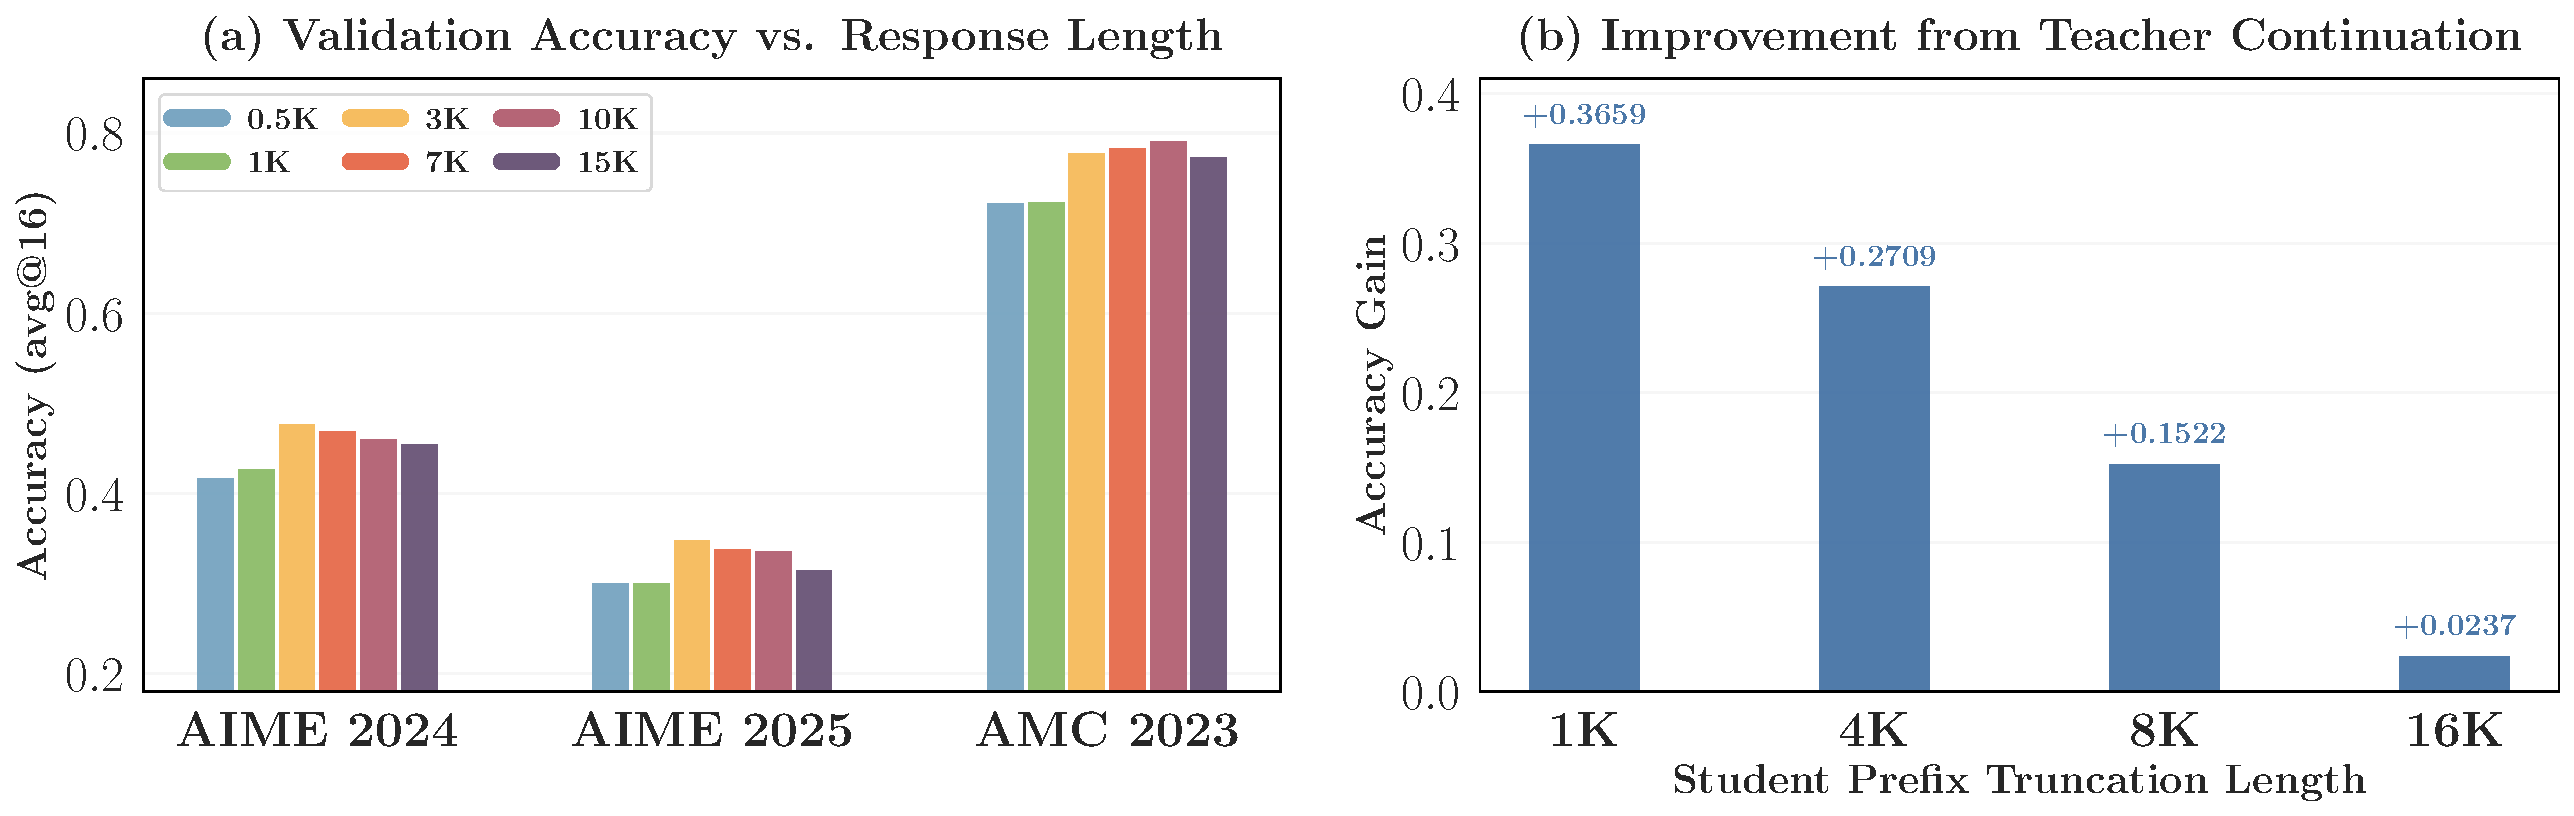
\includegraphics[width=\linewidth]{Figures/6.1.2/6_1_response_summary.pdf}
    \caption{
    (a) Validation accuracy on three benchmarks under different response lengths.
    (b) Accuracy gain from teacher continuation under different student prefix truncation lengths.
    }
    \label{fig:response_length_combined}
\end{figure}

\begin{figure*}[t]
    \centering
    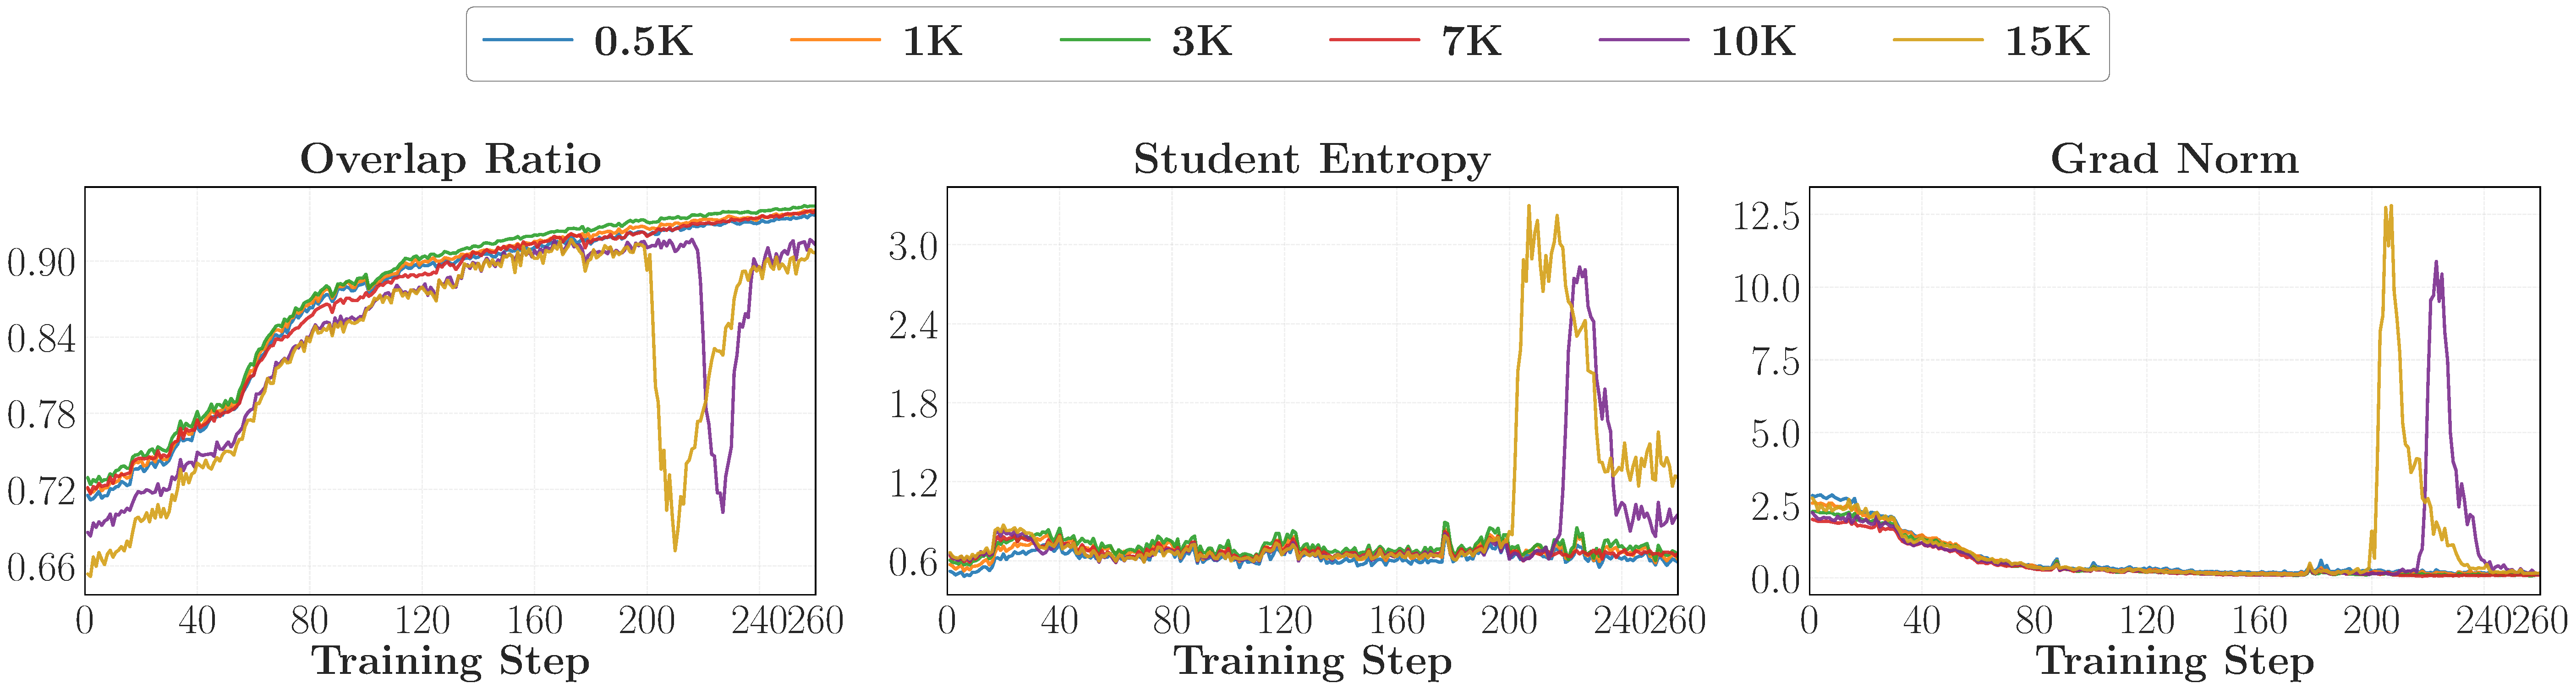
\includegraphics[width=\textwidth]{Figures/6.1.2/6_1_resp_length.pdf}
    \caption{
    Training dynamics under different maximum response lengths for OPD.
    }
    \label{fig:response_length_dynamics}
\end{figure*}

\subsection{Reward Quality Degrades with Trajectory Depth}
\label{sec:reward_noise}


We first investigate how the teacher's reward quality varies with response length.

\paragraph{Response length exhibits a sweet spot.}


The supervision at position $t$ depends on the teacher's conditional $\pi_{T}(y_t \mid x, y_{<t})$ under a student-generated prefix $y_{<t}$, which may drift from trajectories the teacher would naturally produce. We train R1-Distill-1.5B against JustRL-1.5B across six maximum response lengths for 200 steps. As shown in \Cref{fig:response_length_combined}(a), very short responses (0.5K and 1K) provide too few supervised tokens for sample-efficient learning, while moderate lengths (3K and 7K) yield the strongest results. Beyond this range (10K and 15K), performance plateaus or declines. The training dynamics in \Cref{fig:response_length_dynamics} confirm that moderate lengths produce smooth overlap growth, whereas 10K and 15K exhibit late-stage collapse, with the overlap ratio dropping sharply, accompanied by spikes in student entropy and gradient norm.


















\paragraph{Instability originates at later tokens.}
Where does this collapse begin? In the 15K setting, analyzing student entropy as a function of output position across training steps reveals a clear back-to-front pattern: as shown in \Cref{fig:student_entropy_by_position}, high entropy first appears at the end of the response and progressively propagates toward earlier tokens as training proceeds. Teacher entropy exhibits a similar suffix-to-prefix trend (see Appendix~\ref{appendix:teacher_entropy_by_position}), consistent with the teacher encountering increasingly unfamiliar prefixes at later positions and producing noisier reward that in turn destabilizes the student.



\begin{figure*}[t]
    \centering
    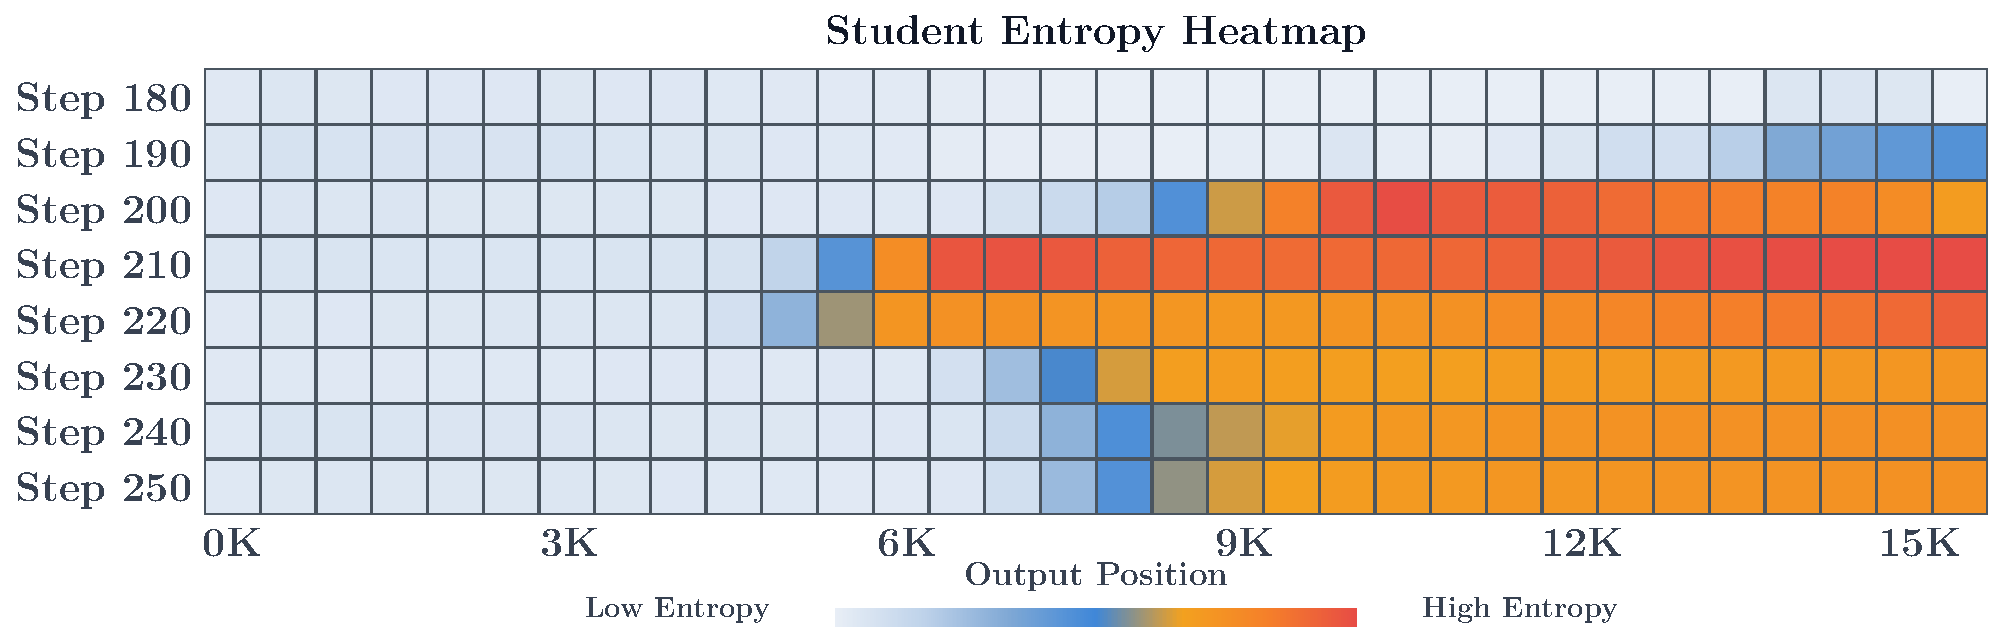
\includegraphics[width=\textwidth]{Figures/4.1/4.1.4/Figure12_student_entropy.pdf}
    \caption{
    Average student entropy across decoding positions during OPD training with 15K max response length, measured on student-generated trajectories from Step 180 to Step 250.
    }
    \label{fig:student_entropy_by_position}
\end{figure*}






\paragraph{Teacher continuation degrades with prefix depth.}
We further probe this by testing whether the teacher can still improve upon the student's continuation when starting from a student-generated prefix. We sample 2K prompts from DAPO-Math-17K, generate full student rollouts, and select those exceeding 16K tokens. We then truncate each rollout at multiple positions and let the teacher continue from the resulting prefix. \Cref{fig:response_length_combined}(b) shows that the teacher’s accuracy advantage decreases monotonically, from +0.37 at a 1K prefix to just +0.02 at a 16K prefix.

Together, these results reveal a fundamental tradeoff in OPD's token-level supervision. Dense reward is effective on moderately long reasoning traces, but its reliability degrades with depth as the student prefix drifts further from the states familiar to the teacher. This suggests that OPD may not extend cleanly to longer-horizon settings such as extended chain-of-thought or agentic multi-turn interaction.












\begin{figure*}[t]
    \centering
    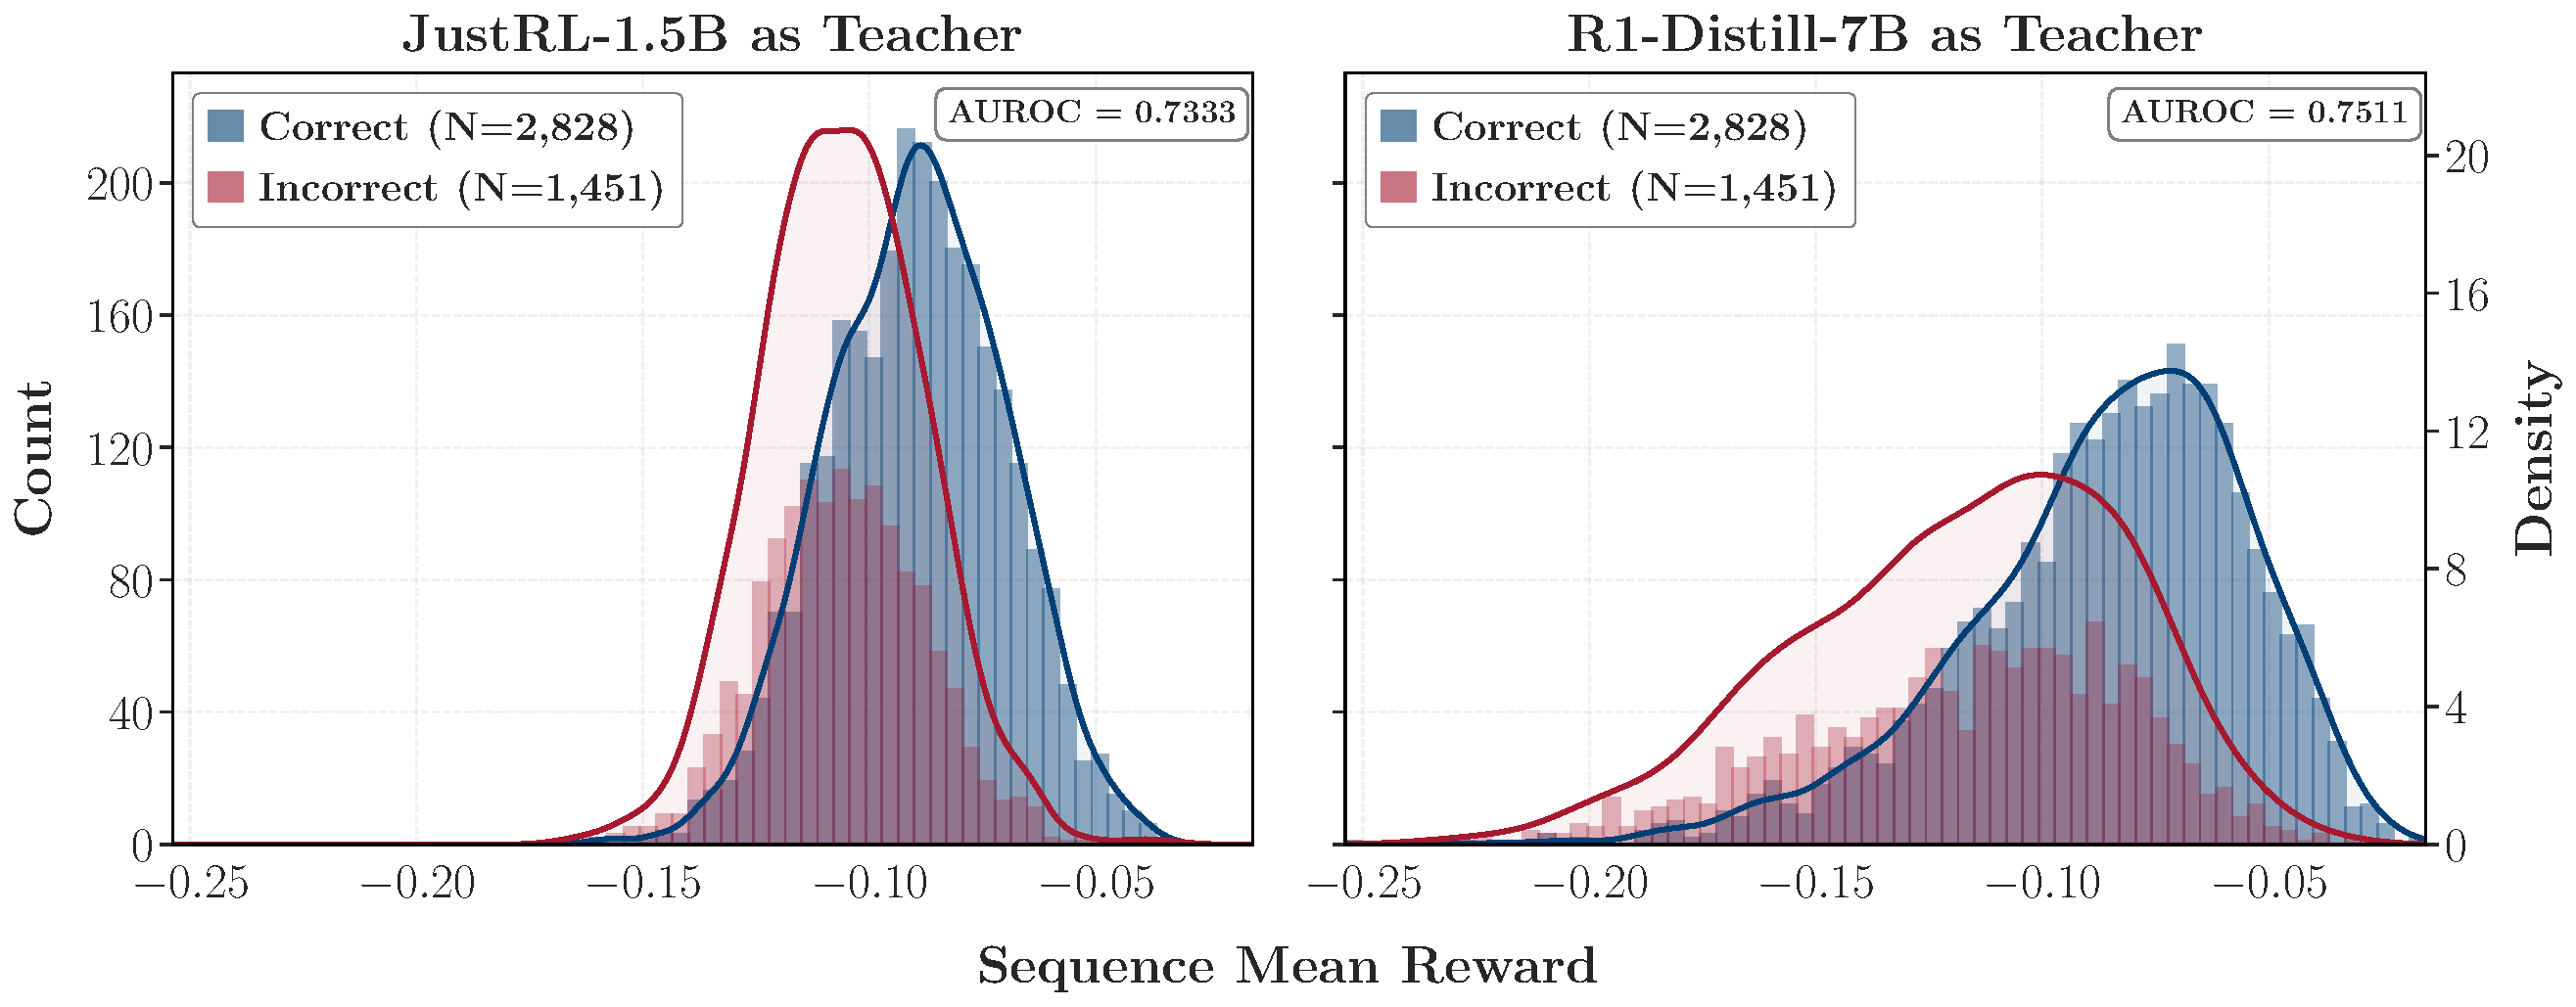
\includegraphics[width=.9\textwidth]{Figures/6.3/reward_landscape.pdf}
    \caption{
    Sequence mean reward distributions for correct and incorrect student rollouts. Both teachers assign higher reward to correct rollouts with comparable AUROC (0.73 and 0.75).
    }
    \label{fig:reward_landscape}
\end{figure*}


\subsection{Globally Informative Reward Does Not Guarantee Local Exploitability}
\label{sec:landscape}





The previous subsection shows that reward quality degrades with trajectory depth. A natural follow-up question is whether the reward signal is fundamentally uninformative in failing OPD configurations or whether the source of failure lies elsewhere.

\paragraph{Setup.}
We revisit the controlled comparison from \Cref{sec:alignment_high_prob}, with R1-Distill-1.5B as the student and two teachers: JustRL-1.5B (successful OPD) and R1-Distill-7B (failed OPD). For each student rollout $y$, we compute the sequence mean reward
$\bar{r}(y) = \frac{1}{T}\sum_{t=1}^{T} \left[\log \pi_{T}(y_t \mid x, y_{<t}) - \log \pi_\theta(y_t \mid x, y_{<t})\right]$
under sampled-token OPD, and compare the distribution of $\bar{r}(y)$ between correct and incorrect rollouts.

\paragraph{Global reward structure is preserved in both settings.}
\Cref{fig:reward_landscape} shows that, for both teachers, correct rollouts consistently receive higher sequence mean reward than incorrect ones, with comparable AUROC values (0.73 for JustRL-1.5B, 0.75 for R1-Distill-7B). The failing 7B teacher does not produce a weaker global signal, which is equally correlated with rollout correctness.

\paragraph{A hypothesis on local optimization geometry.}
If the reward is globally informative in both cases, why does OPD fail with the 7B teacher? The training dynamics from \Cref{sec:alignment_high_prob} offer a clue. As shown in \Cref{fig:alignment_main}, when R1-Distill-7B serves as the teacher, the overlap-token advantage becomes larger in magnitude than in the JustRL setting during the later stages of training, yet the gradient norm remains persistently smaller (see Appendix~\ref{app:auxiliary_dynamics}). One possible explanation is that the 7B teacher's per-token advantages, while individually large, are anisotropic across positions within each sequence. When these heterogeneous signals are aggregated into a gradient update, they partially cancel, yielding small effective gradients despite large per-token rewards. By contrast, JustRL-1.5B, which shares a compatible thinking pattern with the student, may concentrate its advantage on a more coherent subset of tokens. The resulting gradient, though composed of smaller per-token signals, points in a consistent direction that reverse KL can amplify through its mode-seeking behavior.

We have not directly verified this anisotropy hypothesis, and doing so would require analyzing the directional structure of per-token gradients, which we leave to future work. Nonetheless, the co-occurrence of high per-token advantage and low gradient norm is suggestive and points to an important distinction that a globally informative reward does not guarantee a locally exploitable one. Understanding the geometry of OPD's reward landscape, and developing objectives that can exploit anisotropic reward structures, remains an open question.








\subsection{Sampled-Token Reward Is Already Sufficient}
\label{sec:optimal_top_k}

A natural question about OPD's reward is how many tokens per position are needed to compute a useful gradient. Top-$k$ OPD aggregates the reward over the $k$ highest-probability tokens at each position, and one might expect that larger support always leads to better or more stable learning. We investigate this by varying $k$ and comparing against the simpler sampled-token OPD, which uses only a single token drawn from the student distribution at each position.











\begin{figure*}[t]
    \centering
    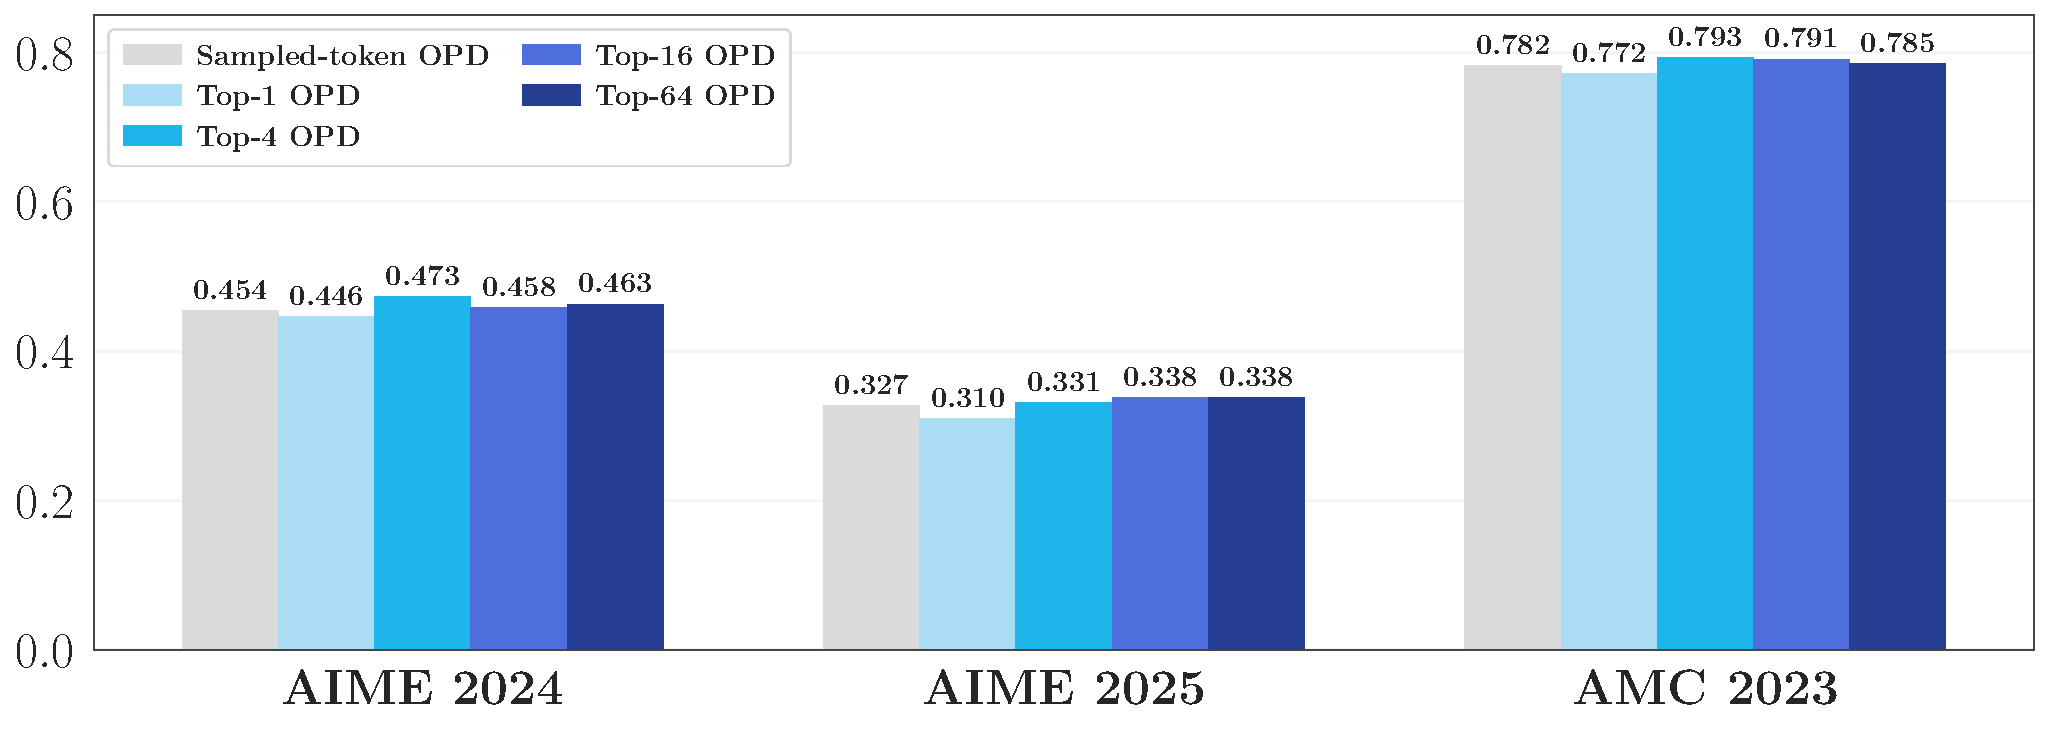
\includegraphics[width=.75\textwidth]{Figures/6.2/5_1_effect_of_k_topk.pdf}
    \caption{Effect of the support size $k$ in Top-$k$ OPD. All numbers are reported as avg@16.}
    \label{fig:effect_of_k_topk}
\end{figure*}


\paragraph{Setup.}
We use R1-Distill-1.5B as the student and JustRL-1.5B as the teacher, and compare Top-$k$ OPD with $k\in\{1, 4, 16, 64\}$ against sampled-token OPD, keeping all other hyperparameters fixed.


\begin{figure*}[t]
    \centering
    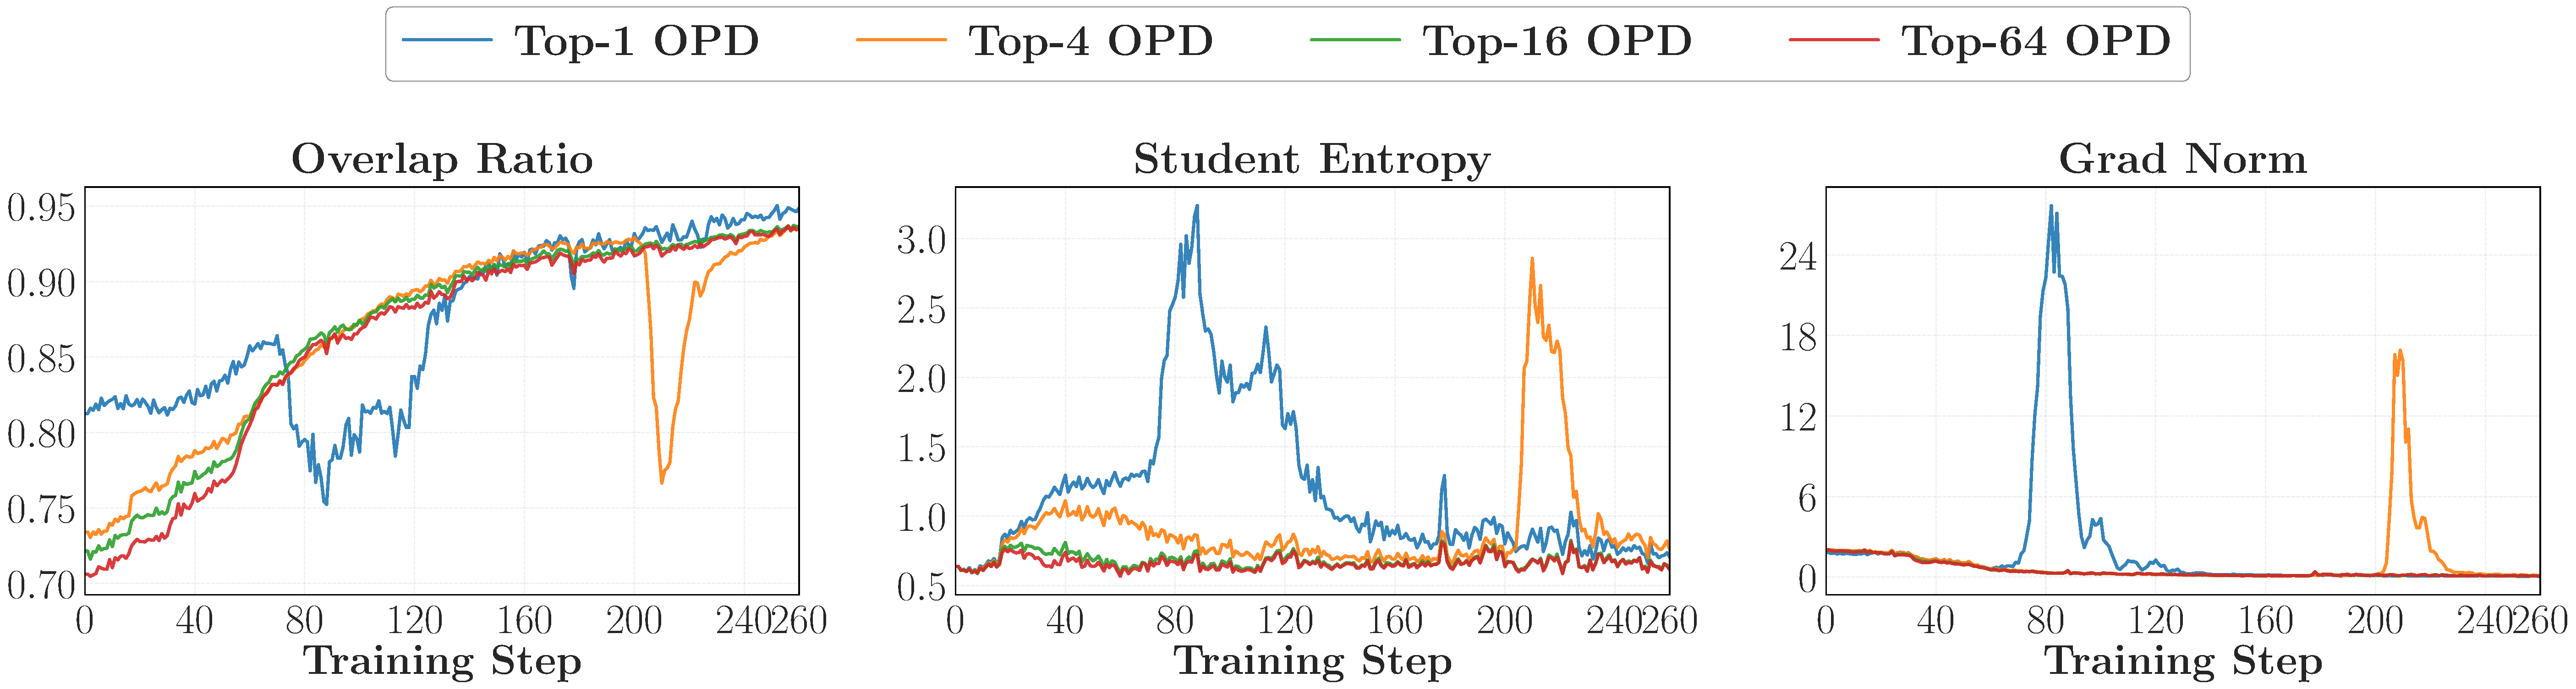
\includegraphics[width=\textwidth]{Figures/6.2/6_2_combined.pdf}
    \caption{Training dynamics under different support sizes $k$ for Top-$k$ OPD.
    }
    \label{fig:effect_of_k_topk_dynamics}
\end{figure*}

\paragraph{Results.}
\Cref{fig:effect_of_k_topk} shows that sampled-token OPD achieves performance comparable to that of the Top-$k$ settings averaged on three benchmarks. The only clearly worse configuration is Top-$1$, which consistently underperforms. Enlarging $k$ beyond 4 brings negligible additional gain while leading to greater computational overhead.
\Cref{fig:effect_of_k_topk_dynamics} shows the training dynamics and reveals where the differences arise. Top-$1$ exhibits unstable overlap growth, accompanied by sharp spikes in entropy and gradient norm. Top-$4$ is substantially more stable but still shows a late-stage dip. Top-$16$ and Top-$64$ remain smooth throughout.

Overall, these results suggest that the support size may not be a critical design choice for OPD, as long as the degenerate Top-$1$ setting is avoided. The reason sampled-token OPD works well despite using only one token per position is that it draws a different token at each step proportionally to the student's own distribution, providing unbiased coverage of the high-probability region across training. Top-$1$, by contrast, always selects the argmax token, thereby concentrating the reward on a single mode. Small policy changes can flip which token occupies rank 1, creating an unstable reward signal that does not average out over training. The failure of Top-$1$ is therefore not about using too few tokens, but about using a biased, mode-concentrated selection rule.






